\documentclass[12pt]{article}

\usepackage{sbc-template}
\usepackage{graphicx,url}
\usepackage[utf8]{inputenc}
\usepackage[brazil]{babel}
%\usepackage[latin1]{inputenc}  

     
\sloppy

\title{Perfil de desempenho e oportunidades de otimização da implementação do método CSEM 3D}

\author{Rômulo T. Lima\inst{1,2}, Mateus F. Lima de Souza\inst{1,3}}

\address{  Laboratório Nacional de Computação Científica (LNCC)\\
  Getúlio Vargas Av., 333, Quitandinha Petrópolis - RJ - Brasil
\nextinstitute
Universidade Católica de Petrópolis (UCP)\\
  R. Barão do Amazonas, 124 - Centro, Petrópolis - RJ - Brasil
\nextinstitute
  Centro Federal de Educação Tecnológica Celso Suckow da Fonseca (CEFET-FR) \\
  R. Gen. Canabarro, 485 - Maracanã, Rio de Janeiro - RJ - Brasil
  \email{\{romulotl,facanha\}@lncc.br}
}

\begin{document} 

\maketitle

\begin{abstract}
  This meta-paper describes the style to be used in articles and short papers
  for SBC conferences. For papers in English, you should add just an abstract
  while for the papers in Portuguese, we also ask for an abstract in
  Portuguese (``resumo''). In both cases, abstracts should not have more than
  10 lines and must be in the first page of the paper.
\end{abstract}
     
\begin{resumo} 
  Este meta-artigo descreve o estilo a ser usado na confecção de artigos e
  resumos de artigos para publicação nos anais das conferências organizadas
  pela SBC. É solicitada a escrita de resumo e abstract apenas para os artigos
  escritos em português. Artigos em inglês deverão apresentar apenas abstract.
  Nos dois casos, o autor deve tomar cuidado para que o resumo (e o abstract)
  não ultrapassem 10 linhas cada, sendo que ambos devem estar na primeira
  página do artigo.
\end{resumo}


\section{Introdução}

\section{CSEM} \label{sec:firstpage}

\section{Processamento Paralelo}
\subsection{HPCToolkit}

\section{Resultados}

\begin{figure}
\centering
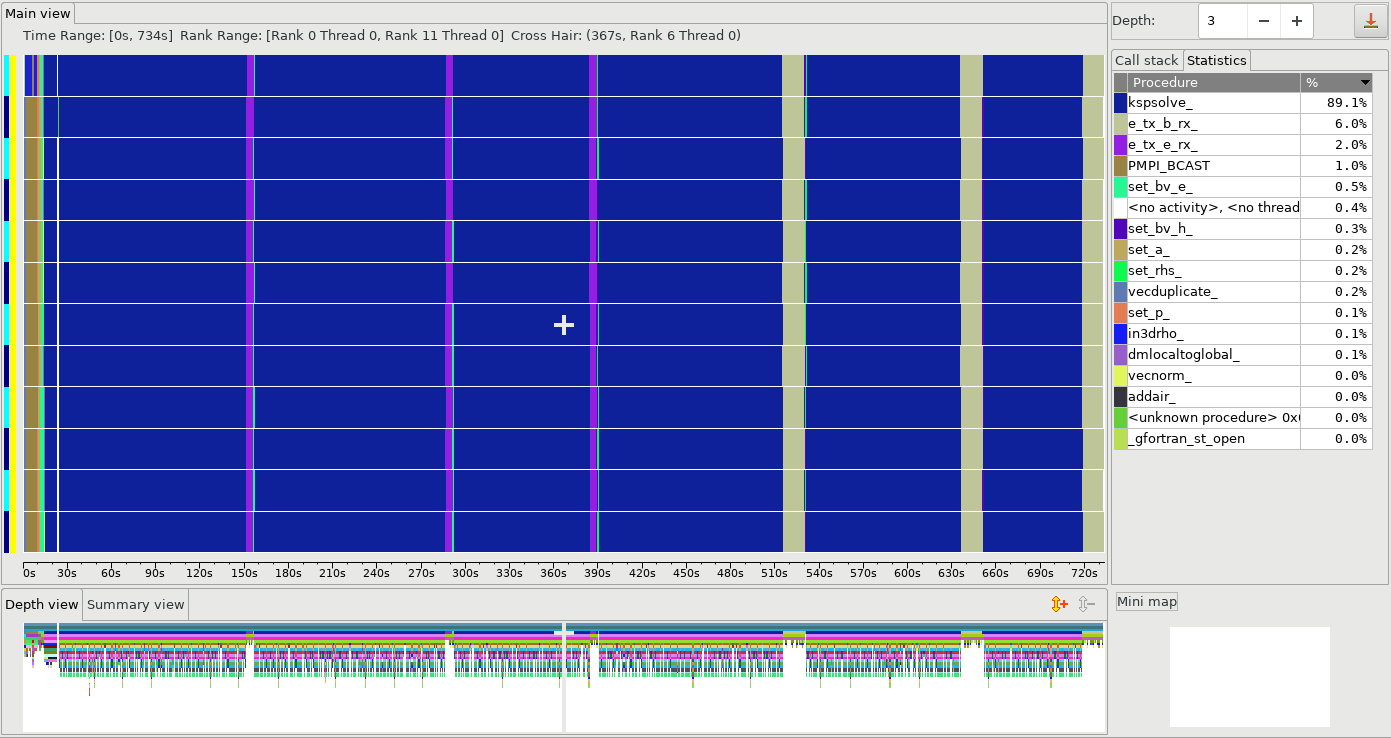
\includegraphics[width=.8\textwidth]{figures/openmpi/Nodes1_MPI12.png}
\caption{HPCToolkit.}
\label{fig:nodes1mpi12}
\end{figure}

\begin{figure}
\centering
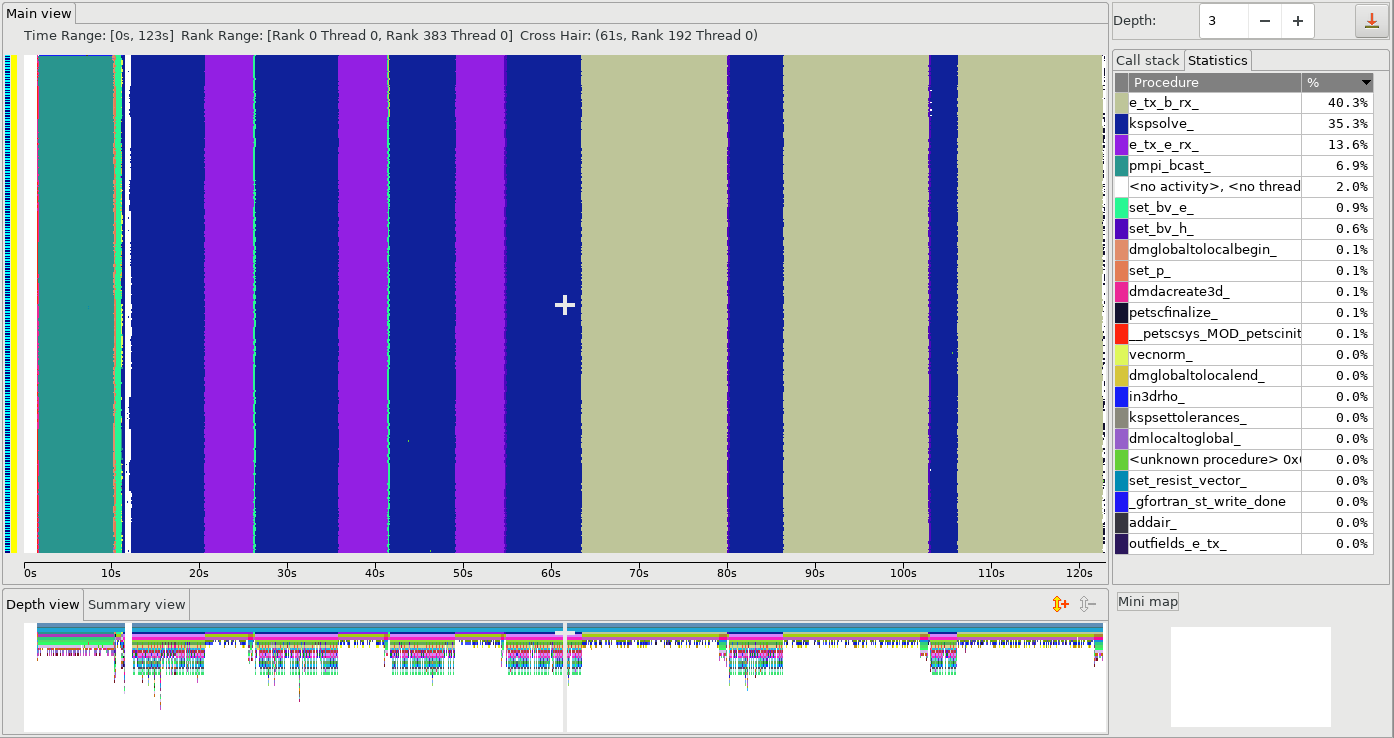
\includegraphics[width=.8\textwidth]{figures/openmpi/Nodes16_MPI384.png}
\caption{HPCToolkit.}
\label{fig:nodes16mpi384}
\end{figure}

\begin{figure}
\centering
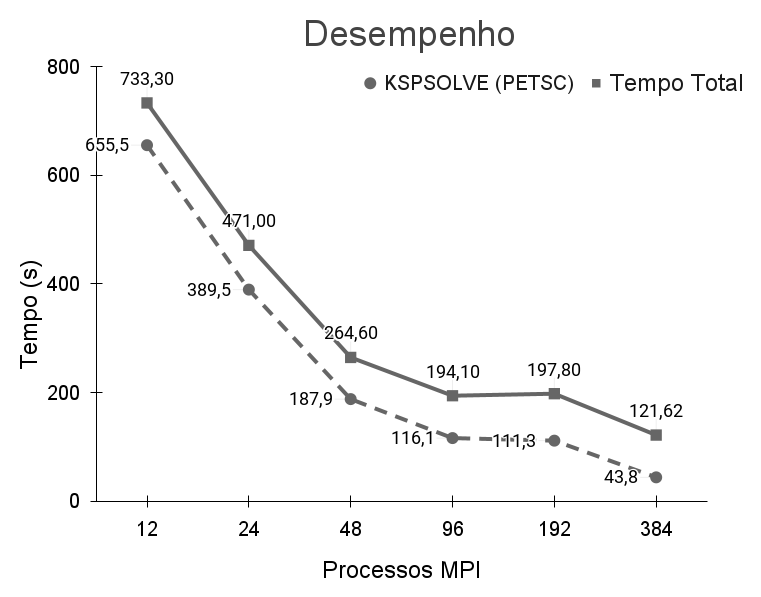
\includegraphics[width=.7\textwidth]{figures/openmpi/desempenho.png}
\caption{Desempenho}
\label{fig:desempenho}
\end{figure}




\section{Comentários}



\section{References}

Bibliographic references must be unambiguous and uniform.  We recommend giving
the author names references in brackets, e.g. \cite{knuth:84},
\cite{boulic:91}, and \cite{smith:99}.

The references must be listed using 12 point font size, with 6 points of space
before each reference. The first line of each reference should not be
indented, while the subsequent should be indented by 0.5 cm.

\bibliographystyle{sbc}
\bibliography{sbc-template}

\end{document}
